\section{Architecture}

%------------------------------------------------
\begin{frame}
	\frametitle{Optimistic concurrency control}
 In a system with \textbf{optimistic concurrency control}, transactions operate under the optimistic assumption that conflicts are rare. 
\vspace{0.5cm}

FoundationDB utilizes \textbf{multiversion concurrency control} as part of its optimistic approach. With MVCC, each transaction operates on a "version" of the data, reflecting a database state at a certain point in time (always a consistent view when reading).
\end{frame}

%------------------------------------------------


\begin{frame}
    \frametitle{Architecture and Transaction Processing}
    \begin{columns}
        \begin{column}{0.5\textwidth}
            \begin{itemize}
                \item \textbf{Control Plane}
                \item \textbf{Data Plane}
                \begin{itemize}
                    \item Transaction System (TS)
                    \item Log System (LS)
                    \item Storage System (SS)
                \end{itemize}
            \end{itemize}
        \end{column}
        \begin{column}{0.5\textwidth}
            \centering
            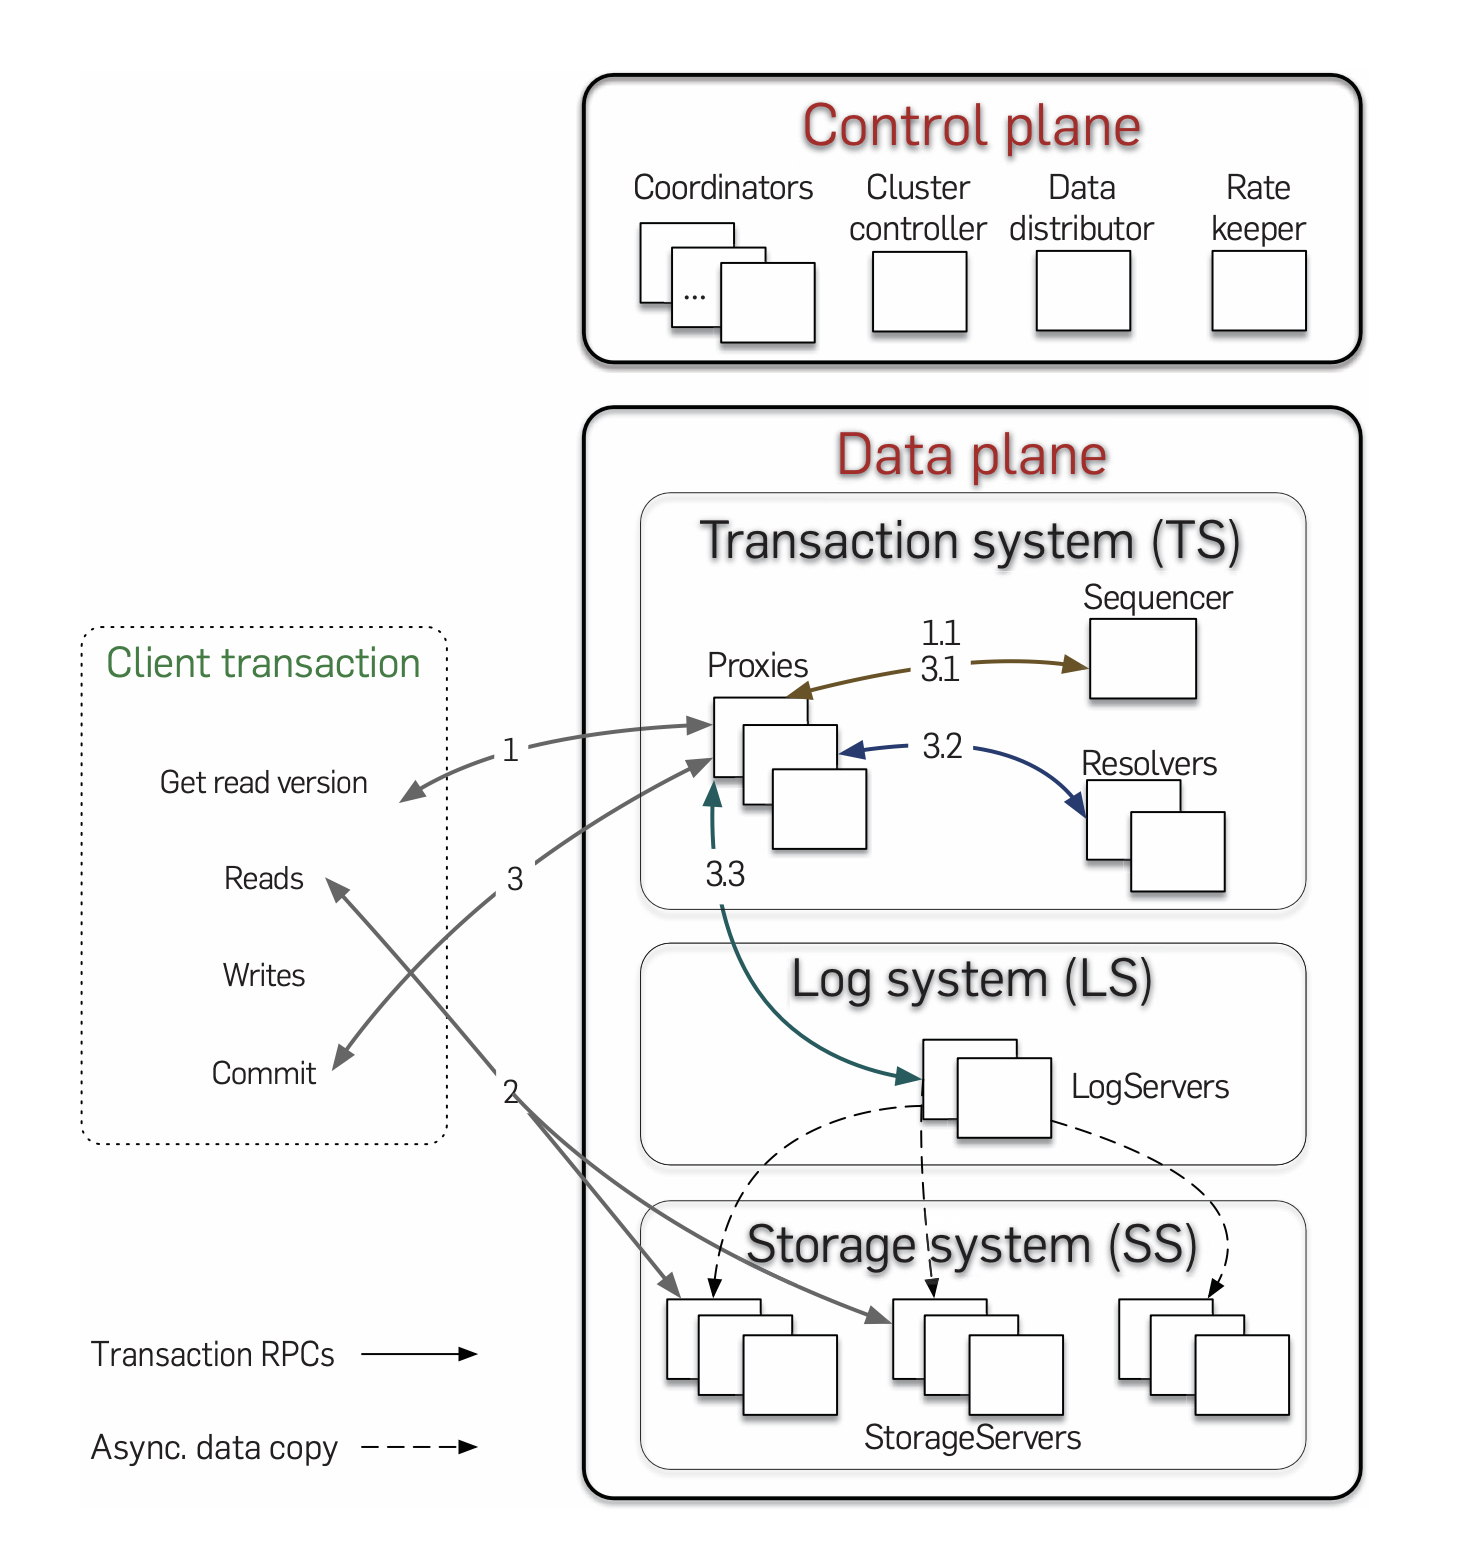
\includegraphics[width=\textwidth]{img/2-Architecture/Architecture and transaction processing.png}
        \end{column}
    \end{columns}
\end{frame}


%------------------------------------------------

% \begin{frame}
% 	\frametitle{Control plane P1}

% The control plane is responsible for persisting critical metadata of the cluster for high availability.
% \textbf{Cluster Controller} monitors all servers in the cluster and recruits 3 processes:
% \begin{itemize}
%     \item Sequencer (Data Plane)
%     \item Data Distributor
%     \item Ratekeeper
% \end{itemize}

% Coordinators form a Paxos group (consensus protocol) and elect the Cluster Controller.
% \end{frame}

%------------------------------------------------


% \begin{frame}
%     \frametitle{Control plane P2}
%     \begin{columns}
%         \begin{column}{0.5\textwidth}
%         \begin{itemize}
%         \item \textbf{Data Distributor} is responsible for monitoring failures and balancing data among Storage Servers.
%         \item \textbf{Ratekeeper} provides overload protection for the cluster.
%         \end{itemize}
        
%         \end{column}
%         \begin{column}{0.5\textwidth}
%             \centering
%             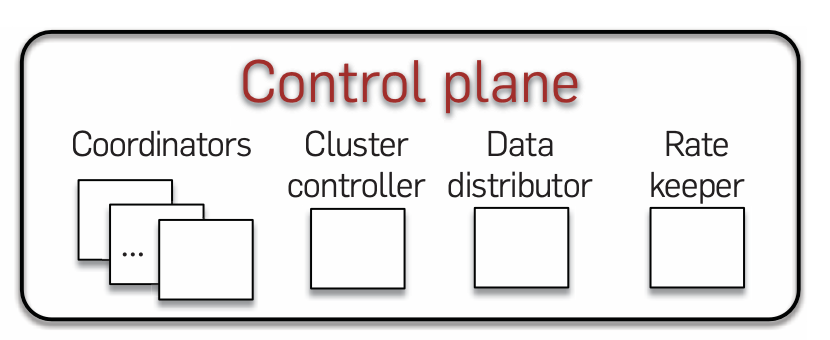
\includegraphics[width=\textwidth]{img/2-Architecture/Control plane.png}
%         \end{column}
%     \end{columns}
% \end{frame}



%------------------------------------------------


\begin{frame}
    \frametitle{Data plane: Transaction system (TS) P1}
    \begin{columns}
        \begin{column}{0.5\textwidth}
        \begin{itemize}
    \item \textbf{Sequencer}: assigns a read and a commit version to each transaction
    \item \textbf{Proxies}: offer MVCC read versions to clients and orchestrate transaction commits
    \item \textbf{Resolvers}: check for conflicts among transactions (5 seconds of history)
   \end{itemize}
        
        \end{column}
        \begin{column}{0.5\textwidth}
            \centering
            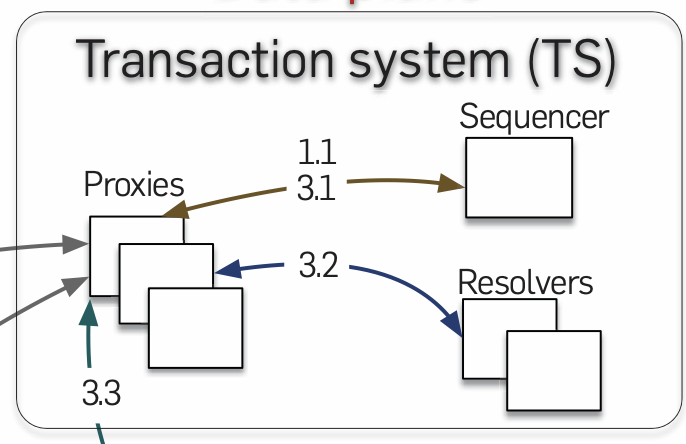
\includegraphics[width=\textwidth]{img/2-Architecture/Transaction System.png}
        \end{column}
    \end{columns}
\end{frame}

%------------------------------------------------

% \begin{frame}
% 	\frametitle{Data plane: Transaction system (TS) P2}

% FoundationDB uses \textbf{multiversion concurrency control} to provide transactionally isolated reads without locking data or blocking writes.
% \vspace{0.5cm}

% \textbf{Optimistic concurrency control} ensures that deadlocks are impossible and that slow or failing clients cannot interfere with the operation of the database.
	
% \end{frame}

% %------------------------------------------------


\begin{frame}
    \frametitle{Data plane: Log system (LS)}
    \begin{columns}
        \begin{column}{0.5\textwidth}
        \textbf{Log Servers} act as replicated, distributed persistent queues, each queue storing "Write-Ahead Log" data for a Storage Server.
        
        \end{column}
        \begin{column}{0.5\textwidth}
            \centering
            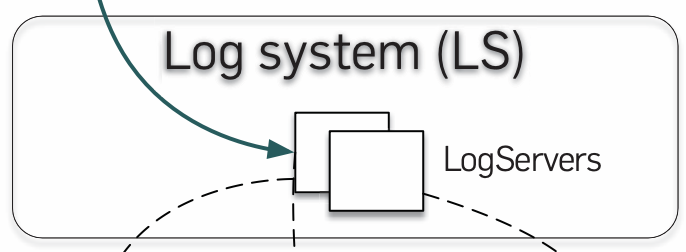
\includegraphics[width=\textwidth]{img/2-Architecture/log system.png}
        \end{column}
    \end{columns}
\end{frame}

% %------------------------------------------------


\begin{frame}
    \frametitle{Data plane: Storage system (SS)}
    \begin{columns}
        \begin{column}{0.5\textwidth}
        The Storage system consists of a number of \textbf{Storage Servers}, each
storing a set of data shards (contiguous key ranges),
and serving client reads. 
\vspace{0.5cm}

Storage Servers are the majority of processes in the system, and together they form a distributed B-tree.
        
        \end{column}
        \begin{column}{0.5\textwidth}
            \centering
            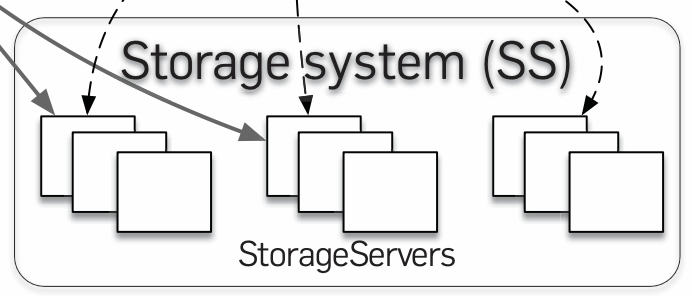
\includegraphics[width=\textwidth]{img/2-Architecture/Storage system.png}
        \end{column}
    \end{columns}
\end{frame}

% %------------------------------------------------
% \begin{frame}
% 	\frametitle{Scaling}
% Scaling is just adding processes for each role. \\

% \begin{itemize}
% \item Clients read from sharded Storage Servers, so reads scale
% linearly with the number of Storage Servers. 
% \end{itemize}

% \vspace{0.5cm}
% Coordinators and control plane's singleton processes like \textbf{Cluster Controller} and \textbf{Sequencer} only perform limited metadata operations.
	
% \end{frame}
% %------------------------------------------------

\begin{frame}
    \frametitle{Transactions: Read}
    \begin{columns}
        \begin{column}{0.5\textwidth}
            \begin{enumerate}
    \item Client $\rightarrow$ Proxies to obtain a read version (timestamp).
    \item Proxy $\rightarrow$ the Sequencer requesting a read version, that is  least as large as all previously issued transaction commit versions.
            \end{enumerate}
        \end{column}
        \begin{column}{0.5\textwidth}
            \centering
            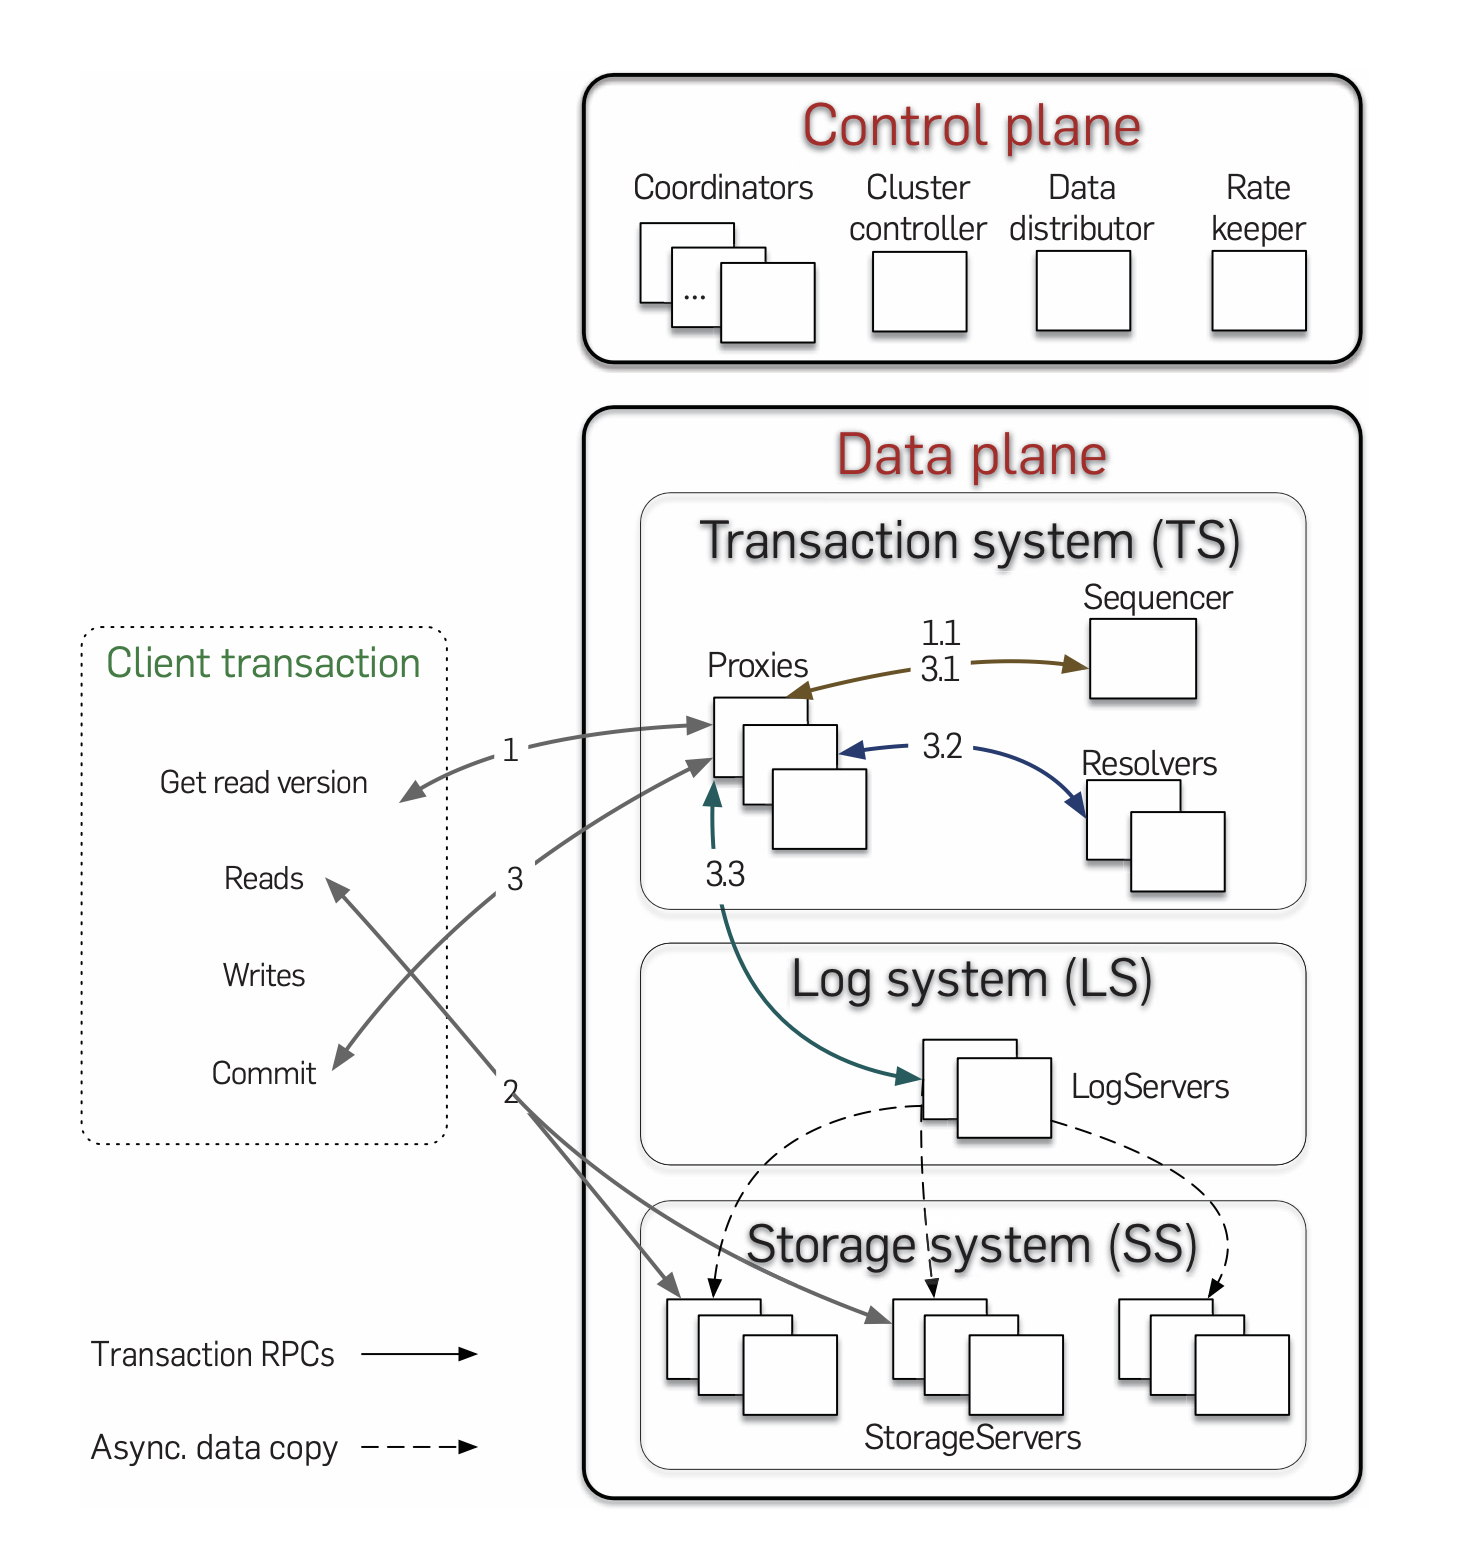
\includegraphics[width=\textwidth]{img/2-Architecture/Architecture and transaction processing.png}
        \end{column}
    \end{columns}
\end{frame}

% %------------------------------------------------

\begin{frame}
    \frametitle{Transactions: Read P2}
    \begin{columns}
        \begin{column}{0.5\textwidth}
            \begin{enumerate}
    \item Proxy $\rightarrow$ client read version.
    \item Client reads from Storage Servers.
    \item Client can cache this information for the next read if needed.
            \end{enumerate}
        \end{column}
        \begin{column}{0.5\textwidth}
            \centering
            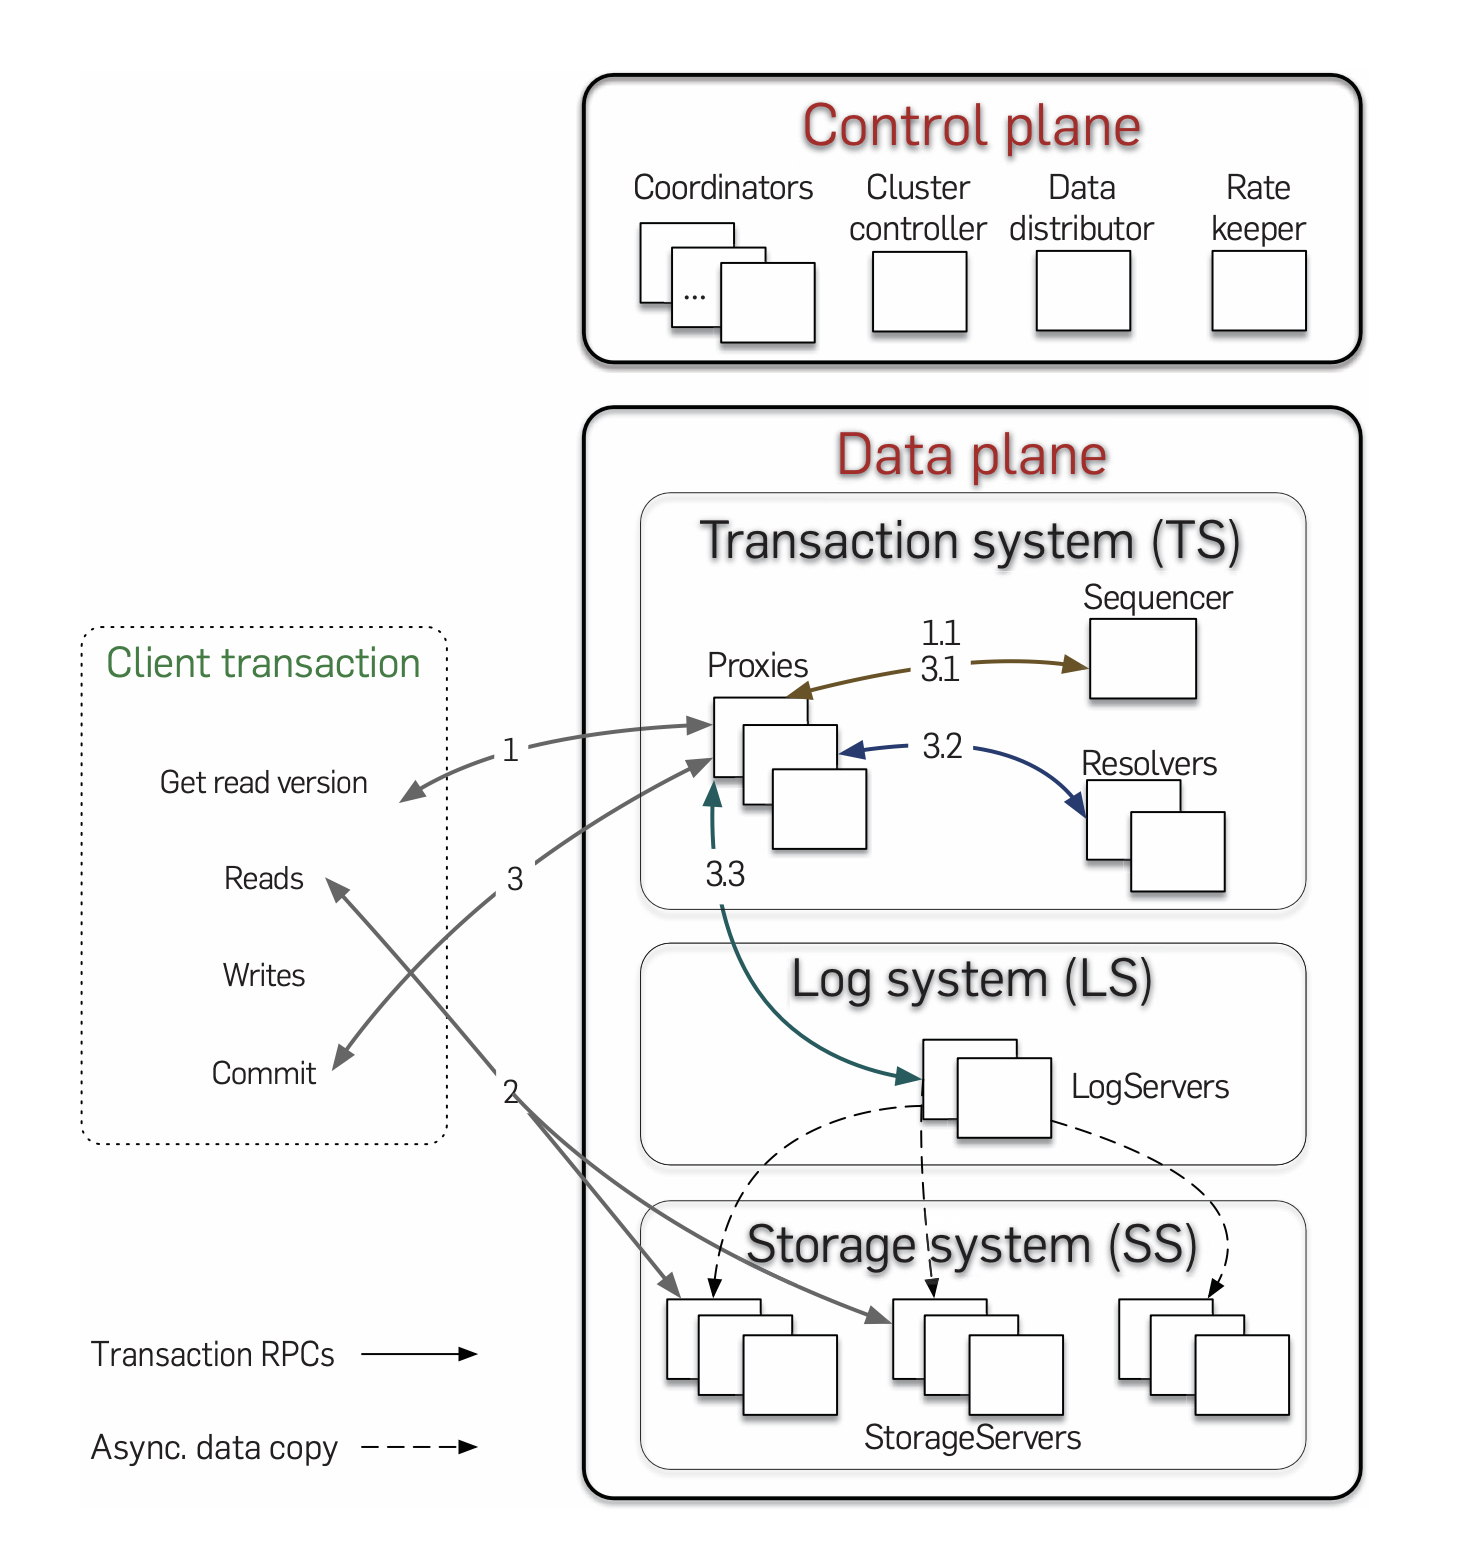
\includegraphics[width=\textwidth]{img/2-Architecture/Architecture and transaction processing.png}
        \end{column}
    \end{columns}
\end{frame}

% %------------------------------------------------

\begin{frame}
    \frametitle{Transactions: Writes}
    \begin{columns}
        \begin{column}{0.5\textwidth}
            \begin{enumerate}
                \item When the client sends the \textbf{transaction data} (read and write that you have done in the transaction) to one of the Proxies
                \item Client waits for a response (commit or abort)
            \end{enumerate}
        \end{column}
        \begin{column}{0.5\textwidth}
            \centering
            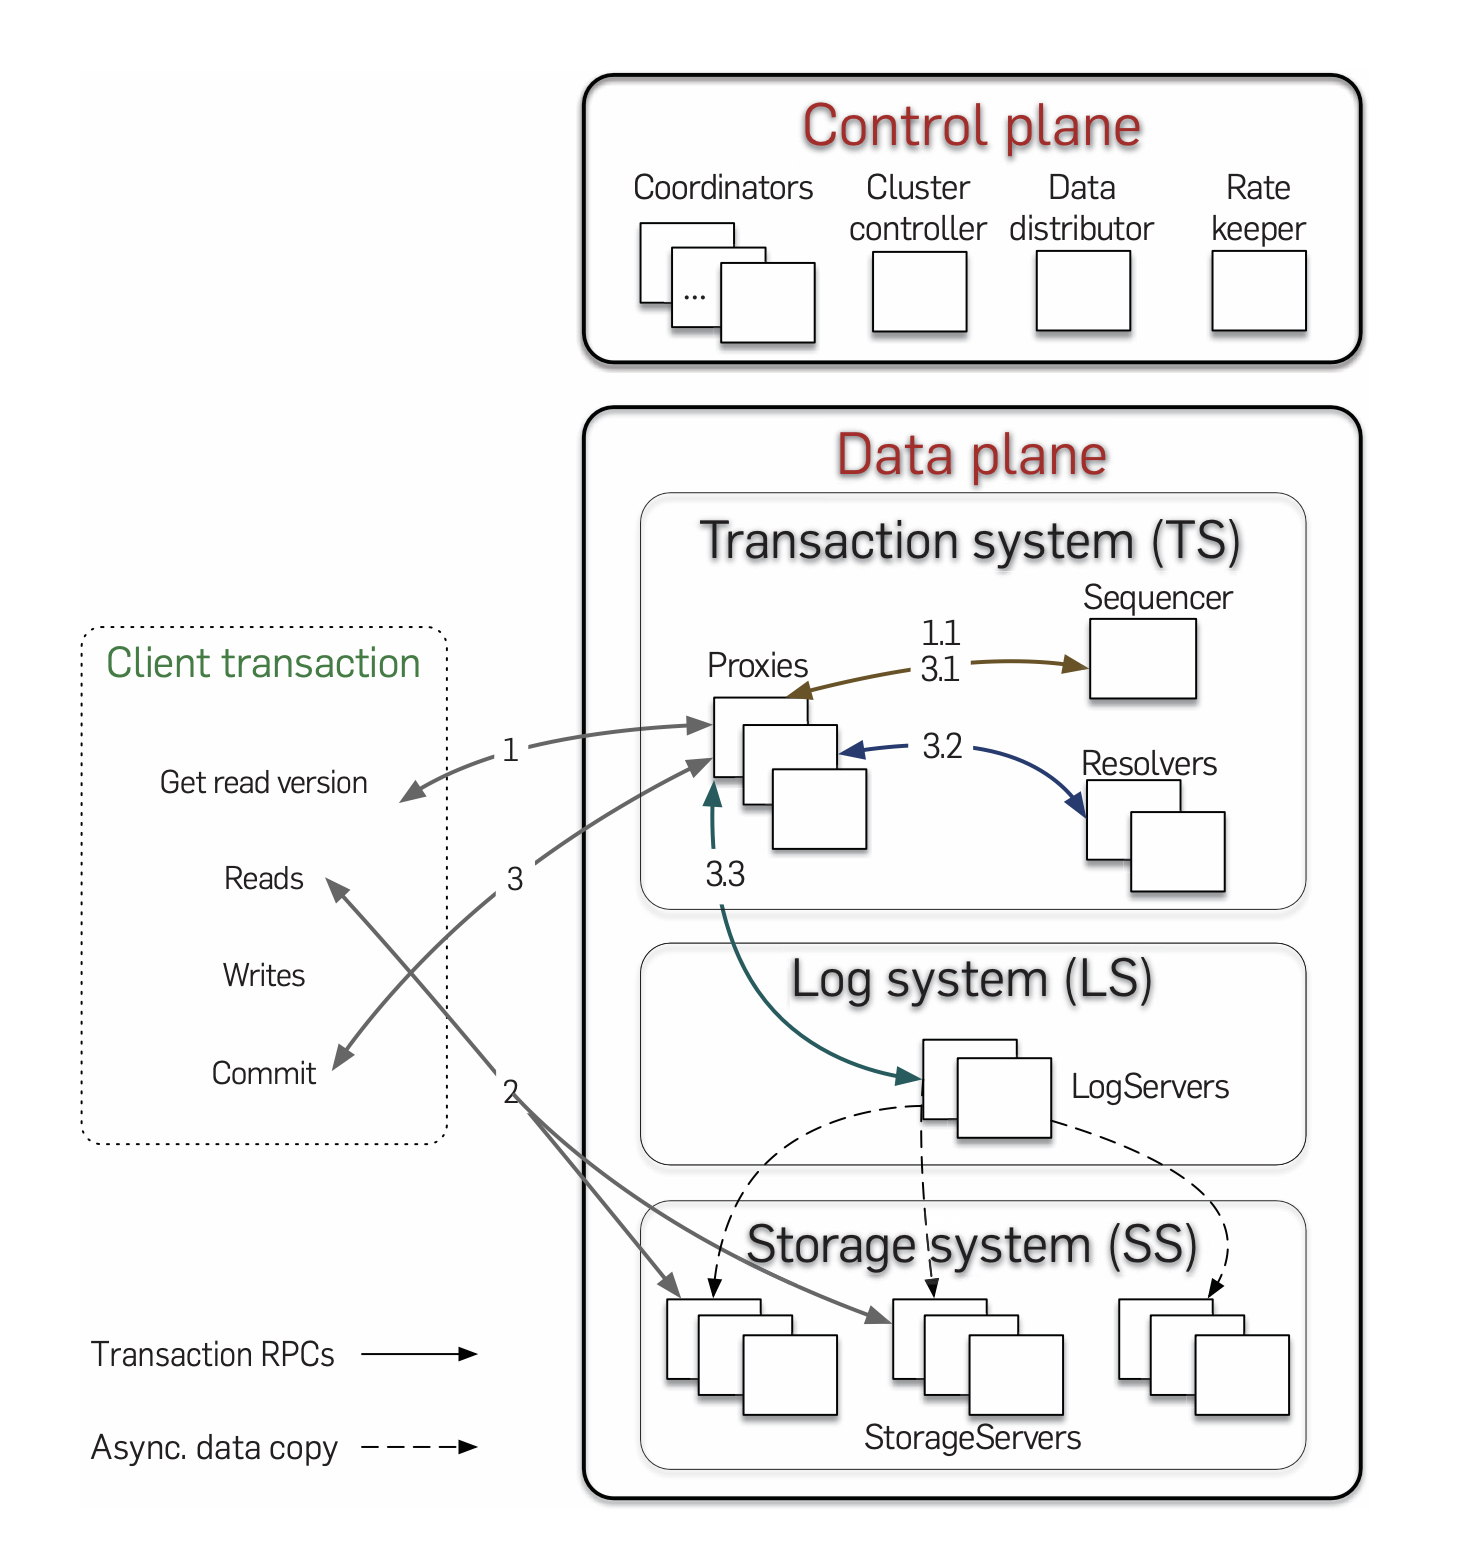
\includegraphics[width=\textwidth]{img/2-Architecture/Architecture and transaction processing.png}
        \end{column}
    \end{columns}
\end{frame}


% %------------------------------------------------
\begin{frame}
    \frametitle{Transactions: Proxy commits}
    \begin{columns}
        \begin{column}{0.5\textwidth}
            \begin{enumerate}
\item Transaction $\rightarrow$ to \textbf{Resolvers} that have to handle the OCC by checking for \b conflicts.
    \item Transaction is forwarded to a set of designated \textbf{Log Servers}.
            \end{enumerate}
        \end{column}
        \begin{column}{0.5\textwidth}
            \centering
            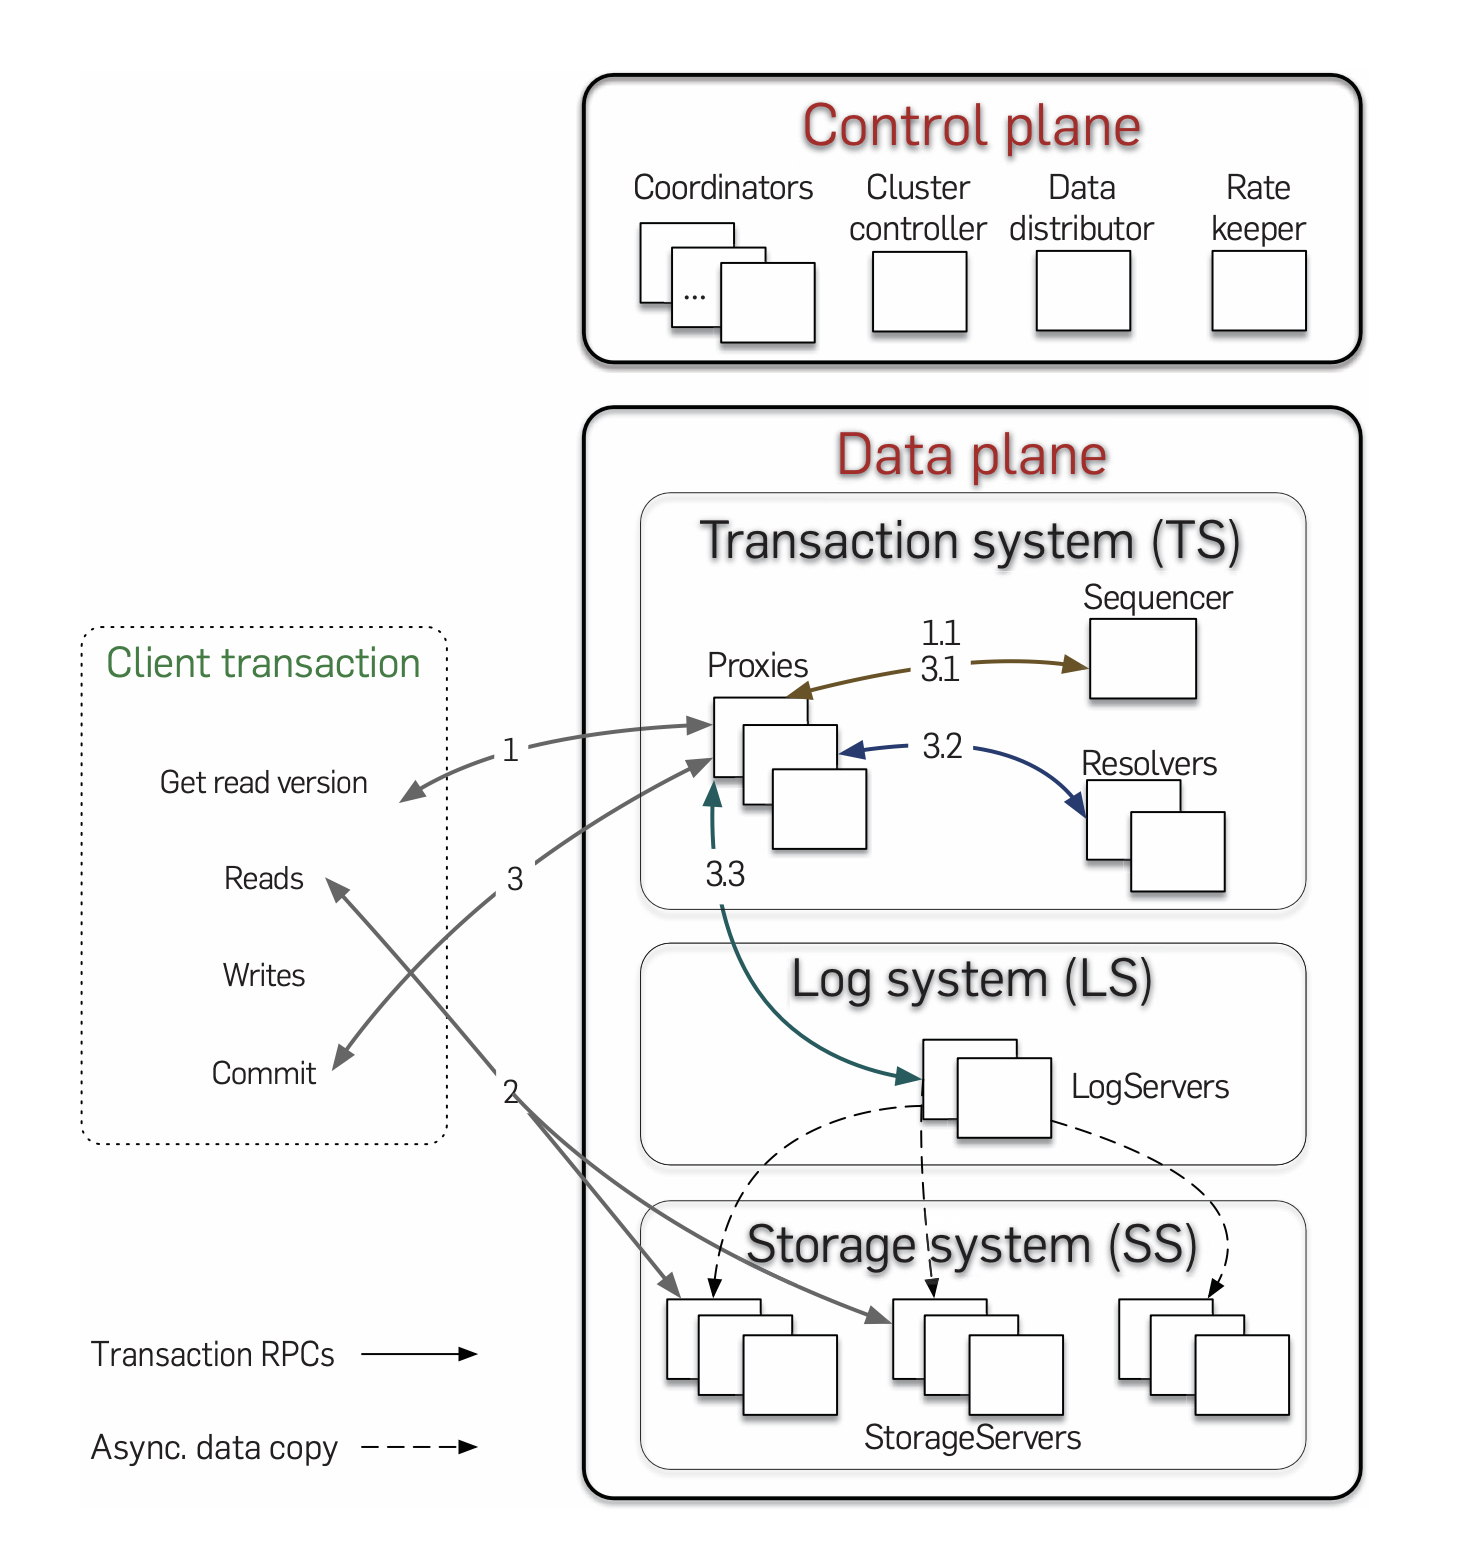
\includegraphics[width=\textwidth]{img/2-Architecture/Architecture and transaction processing.png}
        \end{column}
    \end{columns}
\end{frame}
% %------------------------------------------------
\begin{frame}
    \frametitle{Transactions: Proxy commits P2}
    \begin{columns}
        \begin{column}{0.5\textwidth}
            \begin{enumerate}
    \item Proxy reports the committed version $\rightarrow$ Sequencer, ensures that later transactions' read versions occur after this commit
    \item Proxy replies to the client
            \end{enumerate}
        \end{column}
        \begin{column}{0.5\textwidth}
            \centering
            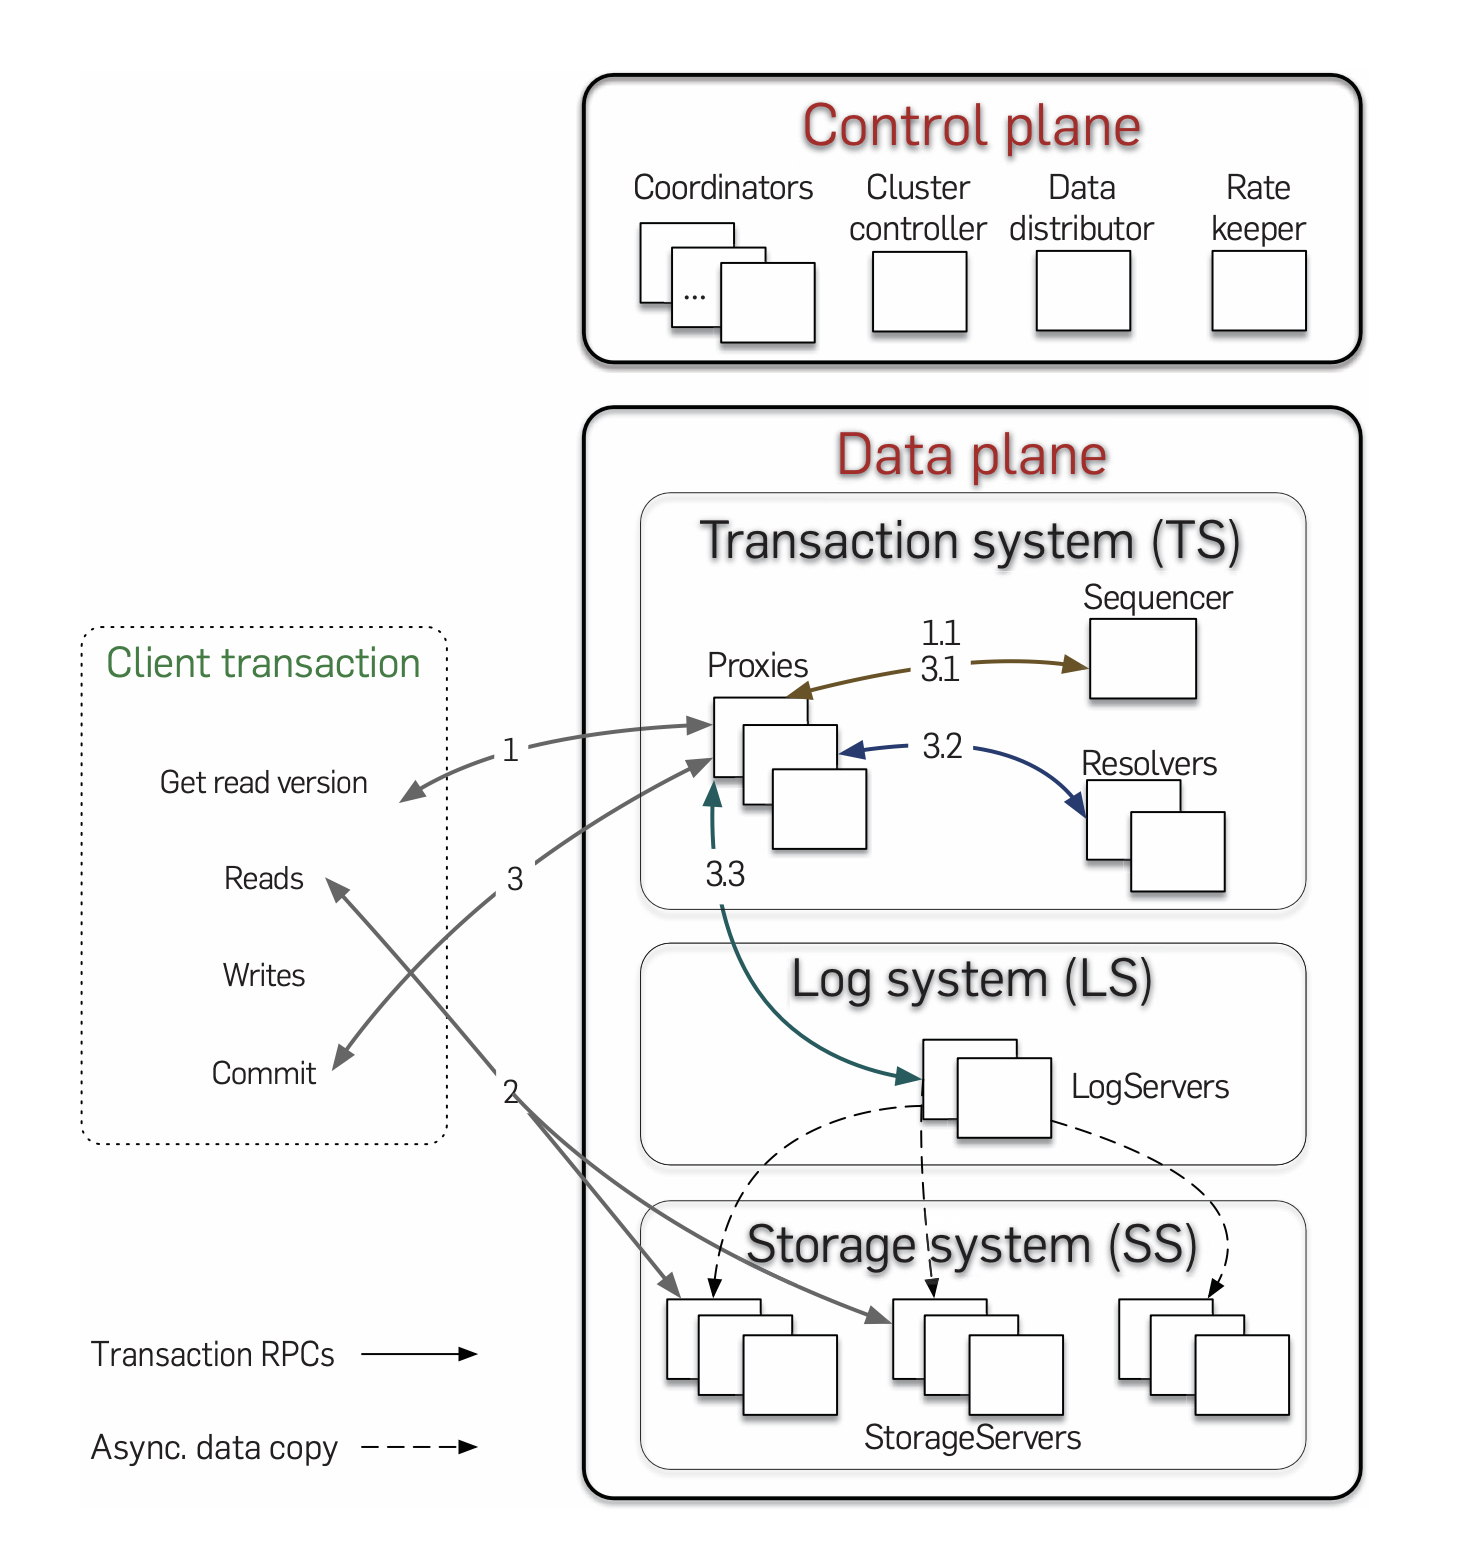
\includegraphics[width=\textwidth]{img/2-Architecture/Architecture and transaction processing.png}
        \end{column}
    \end{columns}
\end{frame}


% %------------------------------------------------


\begin{frame}
	\frametitle{Strict serializability}
\begin{itemize}
  \item FDB ensures strict serializability via Serializable \textbf{Snapshot Isolation} , combining \textbf{OCC} with \textbf{MVCC}.
%   \item Transactions obtain read and commit versions from the Sequencer.
  \item A transaction can commit only when all Resolvers admit the transaction
%   \item The key space is \textbf{divided among Resolvers for parallel conflict detection}.
  \item Optimistic Concurrency Control design \textbf{simplifies TS and SS interactions} but results in \textbf{wasted work for aborted transactions} (client restart the transaction)
\end{itemize}

 \end{frame}


% %------------------------------------------------

\begin{frame}
    \frametitle{Transaction system recover}
    \begin{columns}
        \begin{column}{0.5\textwidth}
            \begin{enumerate}
                \item Traditional databese uses \textbf{ARIES Recovery} (checkpoint, redo, undo).
                \item In FD the recovery is purposely made \textbf{very cheap}, greatly simplifying design choice: \textbf{redo log processing is the same as the normal log forward path}.
                \item System can easily recruit a new TS system in case of failure (Sequencer, Proxies, Resolvers).
            \end{enumerate}
        \end{column}
        \begin{column}{0.5\textwidth}
            \centering
            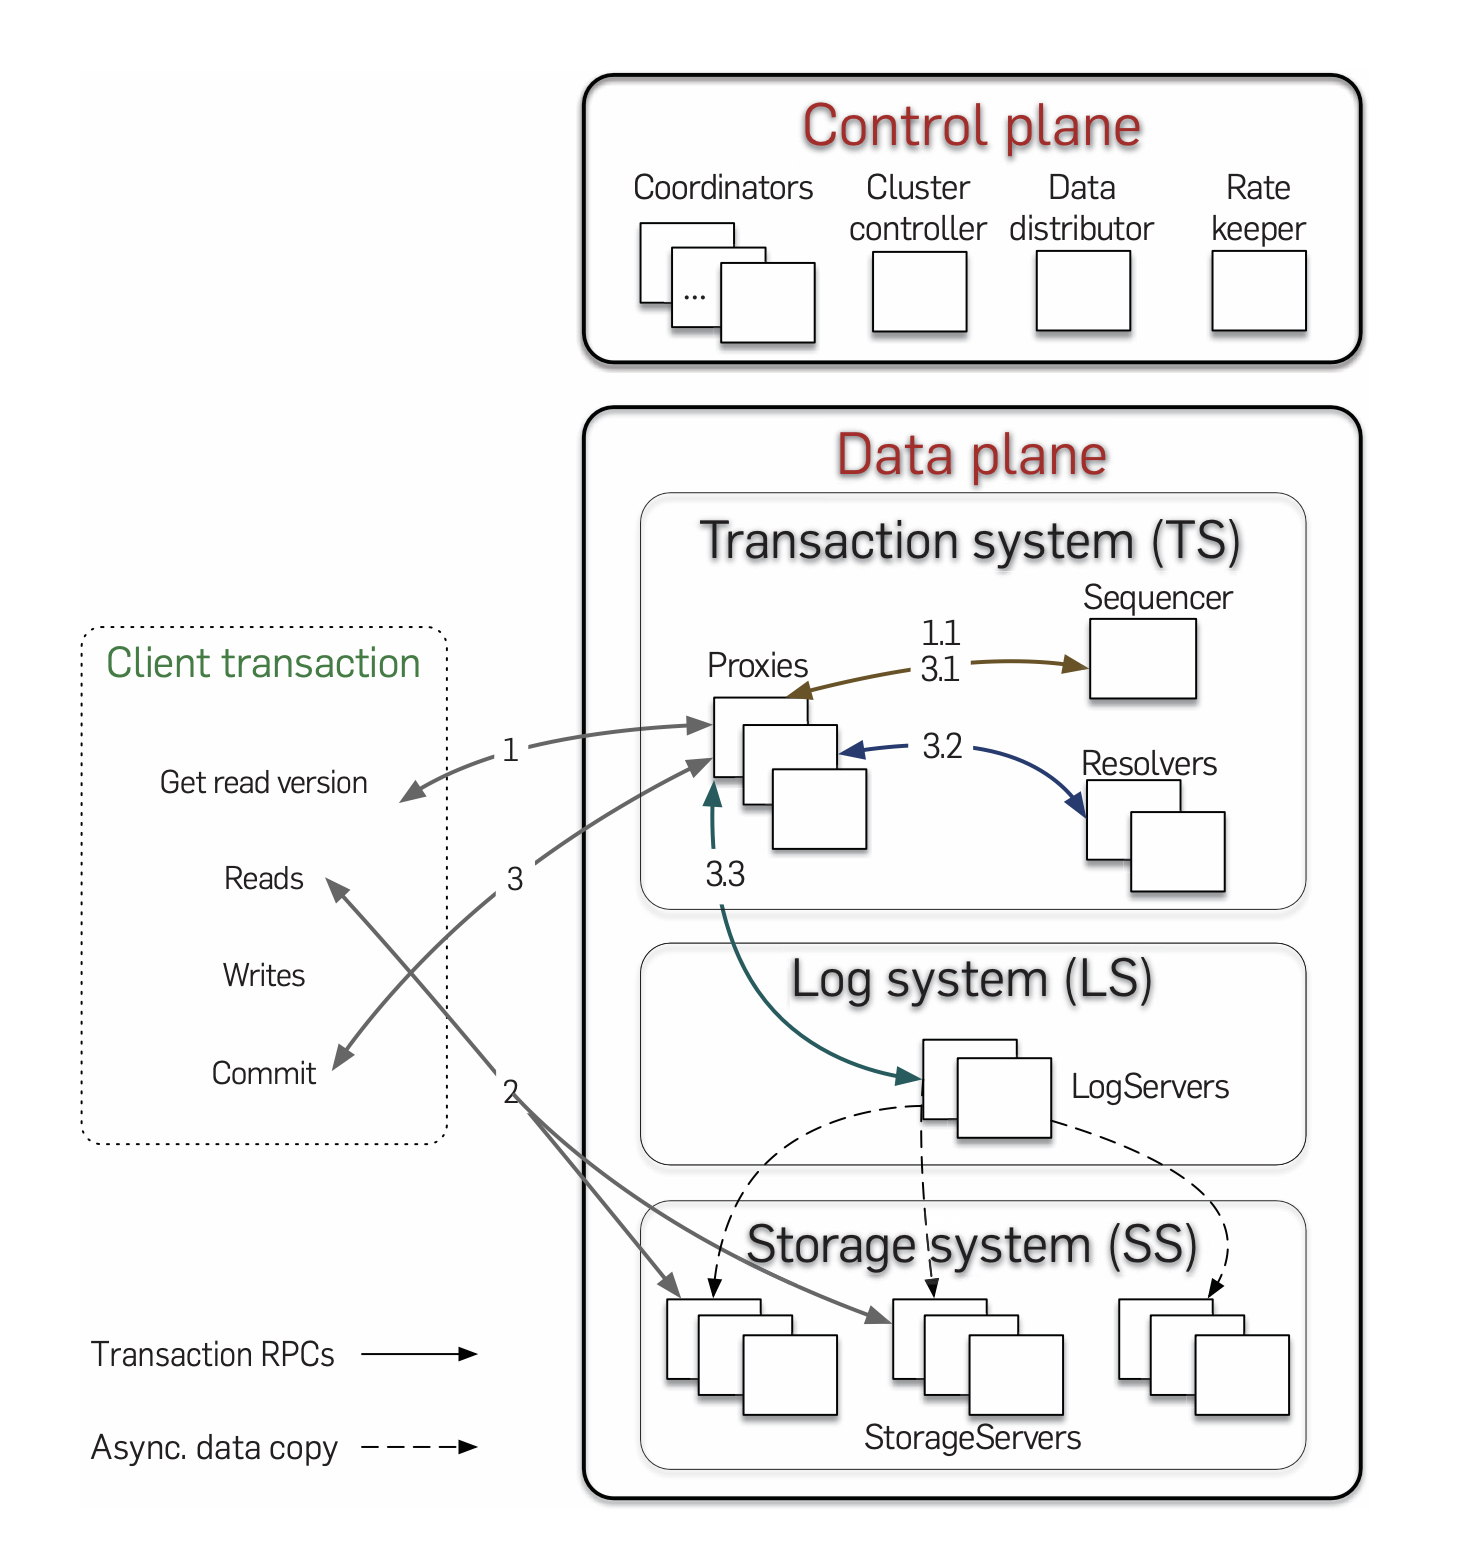
\includegraphics[width=\textwidth]{img/2-Architecture/Architecture and transaction processing.png}
        \end{column}
    \end{columns}
\end{frame}

%------------------------------------------------



% \begin{frame}
% 	\frametitle{Replication: Metadata}
%     \begin{itemize}
%       \item System metadata of the control plane is stored on Coordinators using \textbf{Disk Paxos} (consensus protocol used for reliable data replication across multiple nodes optimized for disk storage)
%       \item As long as a quorum (majority) of Coordinators are live, this metadata can be recovered.

% \end{itemize}
% \end{frame}

 %------------------------------------------------


% \begin{frame}
% 	\frametitle{Replication: Log}
% \begin{itemize}

%       \item When a Proxy writes logs to Log Servers, each sharded log record is synchronously replicated on \textbf{multiple Log Servers}.
%       \item Only when all Log Servers have replied with successful persistence can the Proxy send back the commit response to the client.
%       \item Failure of a Log Server results in \textbf{transaction system recovery}.

% \end{itemize}
% \end{frame}

 %------------------------------------------------


% \begin{frame}
% 	\frametitle{Replication: Storage}
% \begin{itemize}

%       \item Every shard (key range) is asynchronously replicated with multiple Storage Servers, forming a "\textbf{team}".
%       \item A Storage Server usually hosts multiple shards (key range) to evenly \textbf{distribute data across many teams}.
%       \item Failure of a Storage Server triggers Data Distributor to move data from affected teams to healthy ones.

% \end{itemize}
% \end{frame}